
One model to induce word embeddings from (monolingual) text is called \texttt{word2vec}  and was introduced in %REF








Le and Mikolov \cite{Le2014} have extended their monolingual \texttt{word2vec} model to create representations of word sequences (sentences, paragraphs or documents).
It uses a \emph{paragraph vector} as a part of the context of each word in the sequence (Figure~\ref{fig:p2v}). 
This way, the paragraph vector influences the learned representations of those words in the same way that their context words do.

\begin{figure}[here]\center
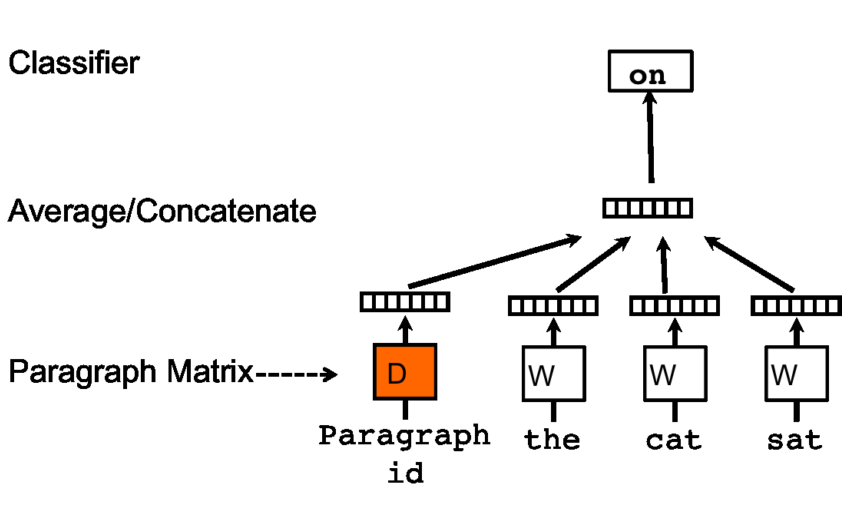
\includegraphics[width=0.7\linewidth]{figures/le.png}
\caption{\texttt{word2vec} for paragraphs}
\label{fig:p2v}
\end{figure}
This paragraph representation could also be used for encouraging similarity between two bitext sentences.
In our novel approach, we will run the algorithm from \cite{Le2014}, but using the same paragraph vector when training word vectors from parallel sentences.
% is dat genoeg? of moet er iets bij over waarom we denken dat de alignments dan niet nodig zijn?
The sentence representation therefore acts as a way to relate the word spaces in both languages, without using word alignments.
% The method is general enough to allow training on more than two sentences. It also encodes more information in the vector than just bag-of-word-vector based models like Herman & Blunsum
We hope this will create a word vector space that is trainable on both monolingual and parallel data, allowing for the mitigation of sparsity in all languages.

% List of different models within this approach as discussed with Philip
We will explore at least two training methods:
\begin{itemize}
\item 
	Sequentially training all sentence pairs. As a paragraph id, we use a single identifier for every sentence pair in the bitext.
	This is equivalent to concatenating the parallel sentences and training from the context windows that do not bridge the sentence boundary.
\item 
	A two-step process:
	First creating paragraph representations for each sentence pair from a fully trained monolingual model. The information from the words in the first language will create a representation for the sentence.
	Then, we fix the sentence representations and train the word spaces in each language using these vectors.
	These sentence vectors will influence the learning of word embeddings in the other languages.
	The error gradient for the sentence vector can either be distributed over the words or be discarded.
\end{itemize}
